% Options for packages loaded elsewhere
\PassOptionsToPackage{unicode}{hyperref}
\PassOptionsToPackage{hyphens}{url}
\PassOptionsToPackage{dvipsnames,svgnames,x11names}{xcolor}
%
\documentclass[
  11pt,
]{article}

\usepackage{amsmath,amssymb}
\usepackage{setspace}
\usepackage{iftex}
\ifPDFTeX
  \usepackage[T1]{fontenc}
  \usepackage[utf8]{inputenc}
  \usepackage{textcomp} % provide euro and other symbols
\else % if luatex or xetex
  \usepackage{unicode-math}
  \defaultfontfeatures{Scale=MatchLowercase}
  \defaultfontfeatures[\rmfamily]{Ligatures=TeX,Scale=1}
\fi
\usepackage{lmodern}
\ifPDFTeX\else  
    % xetex/luatex font selection
    \setmainfont[]{Times New Roman}
\fi
% Use upquote if available, for straight quotes in verbatim environments
\IfFileExists{upquote.sty}{\usepackage{upquote}}{}
\IfFileExists{microtype.sty}{% use microtype if available
  \usepackage[]{microtype}
  \UseMicrotypeSet[protrusion]{basicmath} % disable protrusion for tt fonts
}{}
\makeatletter
\@ifundefined{KOMAClassName}{% if non-KOMA class
  \IfFileExists{parskip.sty}{%
    \usepackage{parskip}
  }{% else
    \setlength{\parindent}{0pt}
    \setlength{\parskip}{6pt plus 2pt minus 1pt}}
}{% if KOMA class
  \KOMAoptions{parskip=half}}
\makeatother
\usepackage{xcolor}
\usepackage[margin=1in]{geometry}
\setlength{\emergencystretch}{3em} % prevent overfull lines
\setcounter{secnumdepth}{5}
% Make \paragraph and \subparagraph free-standing
\makeatletter
\ifx\paragraph\undefined\else
  \let\oldparagraph\paragraph
  \renewcommand{\paragraph}{
    \@ifstar
      \xxxParagraphStar
      \xxxParagraphNoStar
  }
  \newcommand{\xxxParagraphStar}[1]{\oldparagraph*{#1}\mbox{}}
  \newcommand{\xxxParagraphNoStar}[1]{\oldparagraph{#1}\mbox{}}
\fi
\ifx\subparagraph\undefined\else
  \let\oldsubparagraph\subparagraph
  \renewcommand{\subparagraph}{
    \@ifstar
      \xxxSubParagraphStar
      \xxxSubParagraphNoStar
  }
  \newcommand{\xxxSubParagraphStar}[1]{\oldsubparagraph*{#1}\mbox{}}
  \newcommand{\xxxSubParagraphNoStar}[1]{\oldsubparagraph{#1}\mbox{}}
\fi
\makeatother


\providecommand{\tightlist}{%
  \setlength{\itemsep}{0pt}\setlength{\parskip}{0pt}}\usepackage{longtable,booktabs,array}
\usepackage{calc} % for calculating minipage widths
% Correct order of tables after \paragraph or \subparagraph
\usepackage{etoolbox}
\makeatletter
\patchcmd\longtable{\par}{\if@noskipsec\mbox{}\fi\par}{}{}
\makeatother
% Allow footnotes in longtable head/foot
\IfFileExists{footnotehyper.sty}{\usepackage{footnotehyper}}{\usepackage{footnote}}
\makesavenoteenv{longtable}
\usepackage{graphicx}
\makeatletter
\newsavebox\pandoc@box
\newcommand*\pandocbounded[1]{% scales image to fit in text height/width
  \sbox\pandoc@box{#1}%
  \Gscale@div\@tempa{\textheight}{\dimexpr\ht\pandoc@box+\dp\pandoc@box\relax}%
  \Gscale@div\@tempb{\linewidth}{\wd\pandoc@box}%
  \ifdim\@tempb\p@<\@tempa\p@\let\@tempa\@tempb\fi% select the smaller of both
  \ifdim\@tempa\p@<\p@\scalebox{\@tempa}{\usebox\pandoc@box}%
  \else\usebox{\pandoc@box}%
  \fi%
}
% Set default figure placement to htbp
\def\fps@figure{htbp}
\makeatother

\usepackage{xcolor}
\definecolor{navyblue}{RGB}{0, 0, 128}
\definecolor{lightblue}{RGB}{102, 178, 255}

% Title formatting: navy blue, centered, large font
\usepackage{titling}
\pretitle{\begin{center}\Huge\color{navyblue}\bfseries}
\posttitle{\par\end{center}\vskip 0.5em}

% Section and subsection headers color
\usepackage{sectsty}
\sectionfont{\color{lightblue}}      % Sections in light blue
\subsectionfont{\color{lightblue}}   % Subsections in light blue

\makeatletter
\@ifpackageloaded{caption}{}{\usepackage{caption}}
\AtBeginDocument{%
\ifdefined\contentsname
  \renewcommand*\contentsname{Table of contents}
\else
  \newcommand\contentsname{Table of contents}
\fi
\ifdefined\listfigurename
  \renewcommand*\listfigurename{List of Figures}
\else
  \newcommand\listfigurename{List of Figures}
\fi
\ifdefined\listtablename
  \renewcommand*\listtablename{List of Tables}
\else
  \newcommand\listtablename{List of Tables}
\fi
\ifdefined\figurename
  \renewcommand*\figurename{Figure}
\else
  \newcommand\figurename{Figure}
\fi
\ifdefined\tablename
  \renewcommand*\tablename{Table}
\else
  \newcommand\tablename{Table}
\fi
}
\@ifpackageloaded{float}{}{\usepackage{float}}
\floatstyle{ruled}
\@ifundefined{c@chapter}{\newfloat{codelisting}{h}{lop}}{\newfloat{codelisting}{h}{lop}[chapter]}
\floatname{codelisting}{Listing}
\newcommand*\listoflistings{\listof{codelisting}{List of Listings}}
\makeatother
\makeatletter
\makeatother
\makeatletter
\@ifpackageloaded{caption}{}{\usepackage{caption}}
\@ifpackageloaded{subcaption}{}{\usepackage{subcaption}}
\makeatother

\usepackage{bookmark}

\IfFileExists{xurl.sty}{\usepackage{xurl}}{} % add URL line breaks if available
\urlstyle{same} % disable monospaced font for URLs
\hypersetup{
  pdftitle={COVID-19 Impact Analysis: Cases, Deaths, and Vaccination Rates Across Six Countries},
  pdfauthor={Lin Qi, Midhun Unnikrishnan, and Sumintra Boonmat},
  colorlinks=true,
  linkcolor={blue},
  filecolor={Maroon},
  citecolor={Blue},
  urlcolor={blue},
  pdfcreator={LaTeX via pandoc}}


\title{COVID-19 Impact Analysis: Cases, Deaths, and Vaccination Rates
Across Six Countries}
\author{Lin Qi, Midhun Unnikrishnan, and Sumintra Boonmat}
\date{}

\begin{document}
\maketitle

\renewcommand*\contentsname{Table of contents}
{
\hypersetup{linkcolor=}
\setcounter{tocdepth}{3}
\tableofcontents
}

\setstretch{1.5}
\section{Executive Summary}\label{sec-intro}

This report details a study of COVID-19 confirmed cases, deaths, and
vaccination rates across Canada, France, Germany, India, the UK, and the
US from February 2020 to July 2023. It shows the impact of vaccination
on pandemic outcomes. Studies state that countries, including the US and
UK, saw a decrease in both cases and deaths when vaccination uptake
began at the onset of the pandemic. This analysis shows how vaccination
has a proportionately large effect relative to decreasing pandemic
numbers.

\section{Introduction}\label{introduction}

Since early 2020, countries around the globe have experienced COVID-19
to different extents. Governments responded with measures like testing,
lockdowns, and mass vaccination, but the outcomes varied significantly.
This study compares Canada, France, Germany, India, the UK, and the US
to understand the contrast in outcomes. It researches time series data
on confirmed cases, deaths, and vaccination rates from 2020 to 2023. The
primary question focuses on the role of vaccination in decreasing case
numbers and mortality rates. Vaccination programs started at varying
times, with richer nations beginning earlier. For example, Canada and
the United States started vaccinations in December 2020, while India
began in January 2021. This study aims to provide insight into
successful responses to the pandemic. It highlights the importance of
vaccination in reducing the spread and severity of the virus.

\section{Methodology}\label{sec-method}

\textbf{Data Source}:

We used publicly available datasets from
\href{https://ourworldindata.org/coronavirus}{Our World in Data},
including:

\begin{itemize}
\item
  Confirmed COVID-19 case numbers:
  https://ourworldindata.org/covid-cases
\item
  COVID-19 death data: https://ourworldindata.org/covid-deaths
\item
  COVID-19 vaccination data:
  https://ourworldindata.org/covid-vaccinations
\end{itemize}

\textbf{Time Range Validation}:

\begin{itemize}
\item
  Confirmed Cases: February 1, 2020 - February 1, 2023
\item
  Death Rates: February 1, 2020 - February 1, 2023
\item
  Vaccination Data:
\end{itemize}

The vaccination dataset was obtained from Our World in Data. We observed
that different countries had different vaccination start and end dates.
For example, Canada and the US began recording vaccinations in December
2020, while India started in mid-January 2021. These differences are
likely due to unequal access to vaccines and different national data
reporting schedules.

To ensure fair comparisons, we limited our analysis to the overlapping
period across all six countries: from January 16, 2021 to September 4,
2022. This allows for consistent visualization and avoids bias caused by
missing early or late-stage data in certain countries.

\textbf{Data Cleaning and Preprocessing}:

Before analysis, we checked for missing values in the vaccination
dataset. We removed any records with missing doses per million using R's
\texttt{filter(!is.na(...))} function.

We then merged the confirmed case dataset with the vaccination dataset
by country and date. To ensure valid comparisons across countries, we
filtered the merged dataset to include only the common time range where
all countries had vaccination data available.

\begin{figure}

\centering{

\pandocbounded{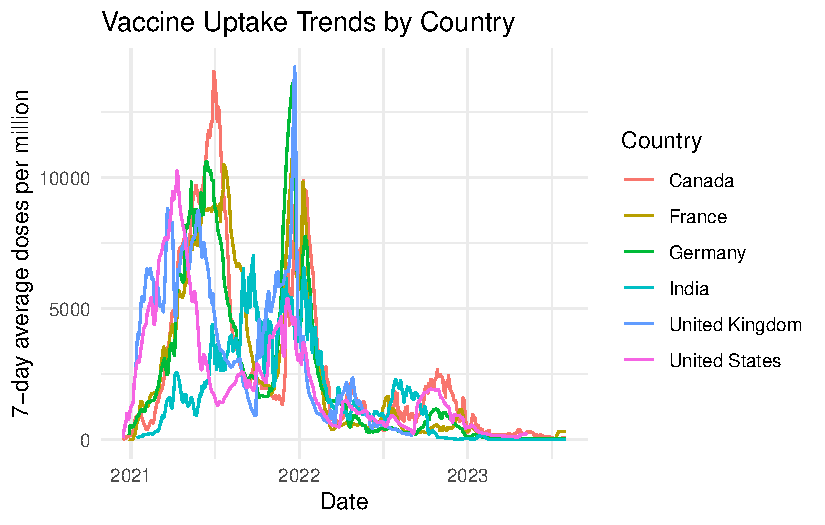
\includegraphics[keepaspectratio]{Analysis_files/figure-pdf/fig-vacc-trend-1.pdf}}

}

\caption{\label{fig-vacc-trend}Figure: COVID-19 vaccine: 7-day average
doses per million (by country)}

\end{figure}%

\begin{longtable}[]{@{}lll@{}}

\caption{\label{tbl-vacc-summary}Table: Summary of vaccination data
coverage (start-end date by country)}

\tabularnewline

\toprule\noalign{}
Country & Start & End \\
\midrule\noalign{}
\endhead
\bottomrule\noalign{}
\endlastfoot
Canada & 2020-12-15 & 2023-07-31 \\
France & 2020-12-28 & 2023-07-31 \\
Germany & 2020-12-28 & 2023-07-31 \\
India & 2021-01-16 & 2023-07-31 \\
United Kingdom & 2021-01-11 & 2022-09-04 \\
United States & 2020-12-15 & 2023-05-09 \\

\end{longtable}

Figure~\ref{fig-vacc-trend} shows the 7-day average vaccination doses
per million across the six countries. Canada, France, Germany, the UK,
and the US all ramped up vaccination rapidly during early 2021, while
India lagged slightly behind, with a noticeable delay in rollout.
Table~\ref{tbl-vacc-summary} confirms the start and end dates of vaccine
data coverage, showing that most countries began vaccination efforts in
late December 2020. This aligns with Our World in Data's findings that
vaccine rollout was uneven globally, with lower coverage in lower-income
regions.

\begin{figure}

\centering{

\pandocbounded{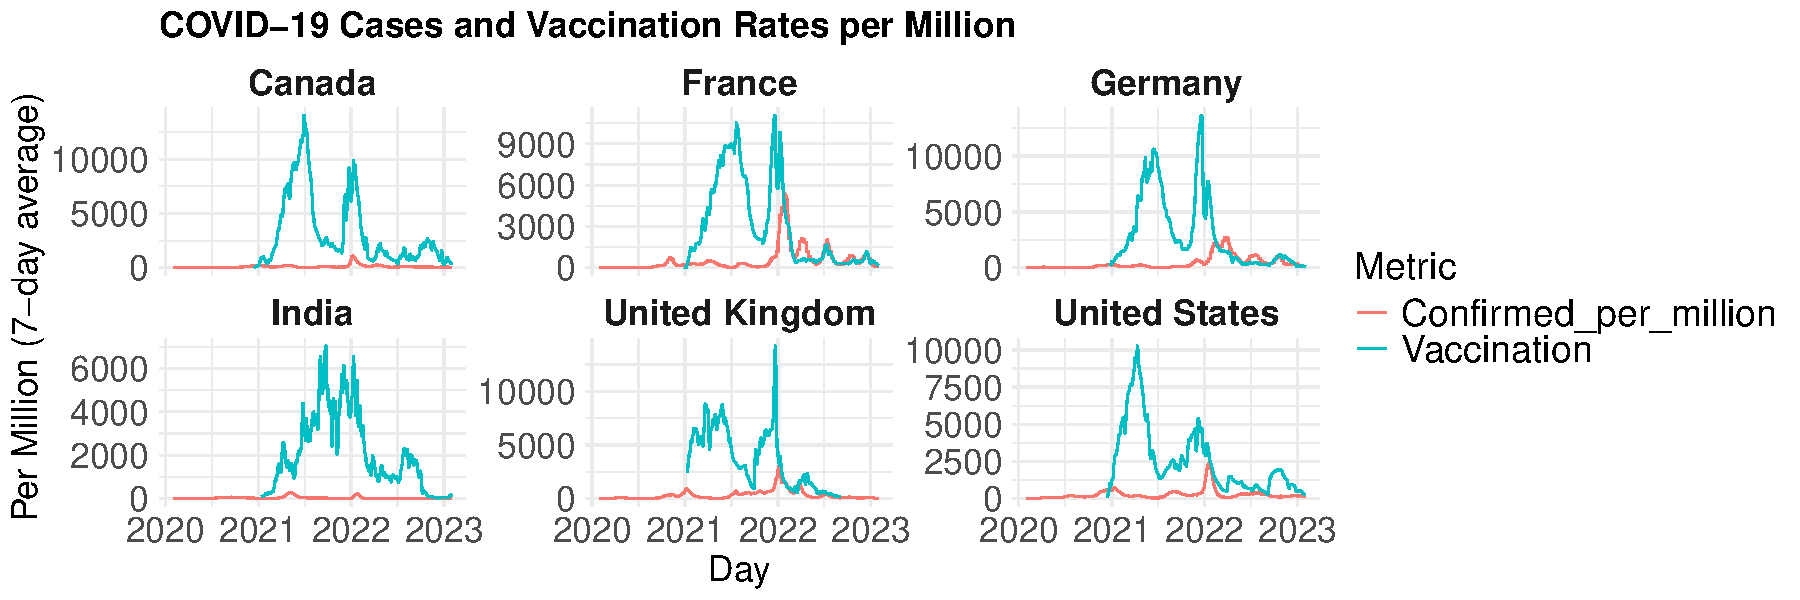
\includegraphics[keepaspectratio]{Analysis_files/figure-pdf/fig-vacc-vs-case-1.pdf}}

}

\caption{\label{fig-vacc-vs-case}Figure: Comparison of confirmed cases
and vaccination rates per million (by country)}

\end{figure}%

In order to more clearly understand the temporal relationship between
COVID-19 outbreaks and vaccination, we constructed the
Figure~\ref{fig-vacc-vs-case}, which displays the number of daily
diagnoses per million people overlaid on the number of vaccinations,
arranged faceted by country. We can see that the number of confirmed
cases increased before the vaccination rate started to rise. This means
that many governments began to roll out vaccines after the number of
cases went up. This figure is useful for visualizing the timing between
outbreaks and vaccination responses. It helps us see whether vaccines
were given early or late during a wave.

\begin{figure}

\centering{

\pandocbounded{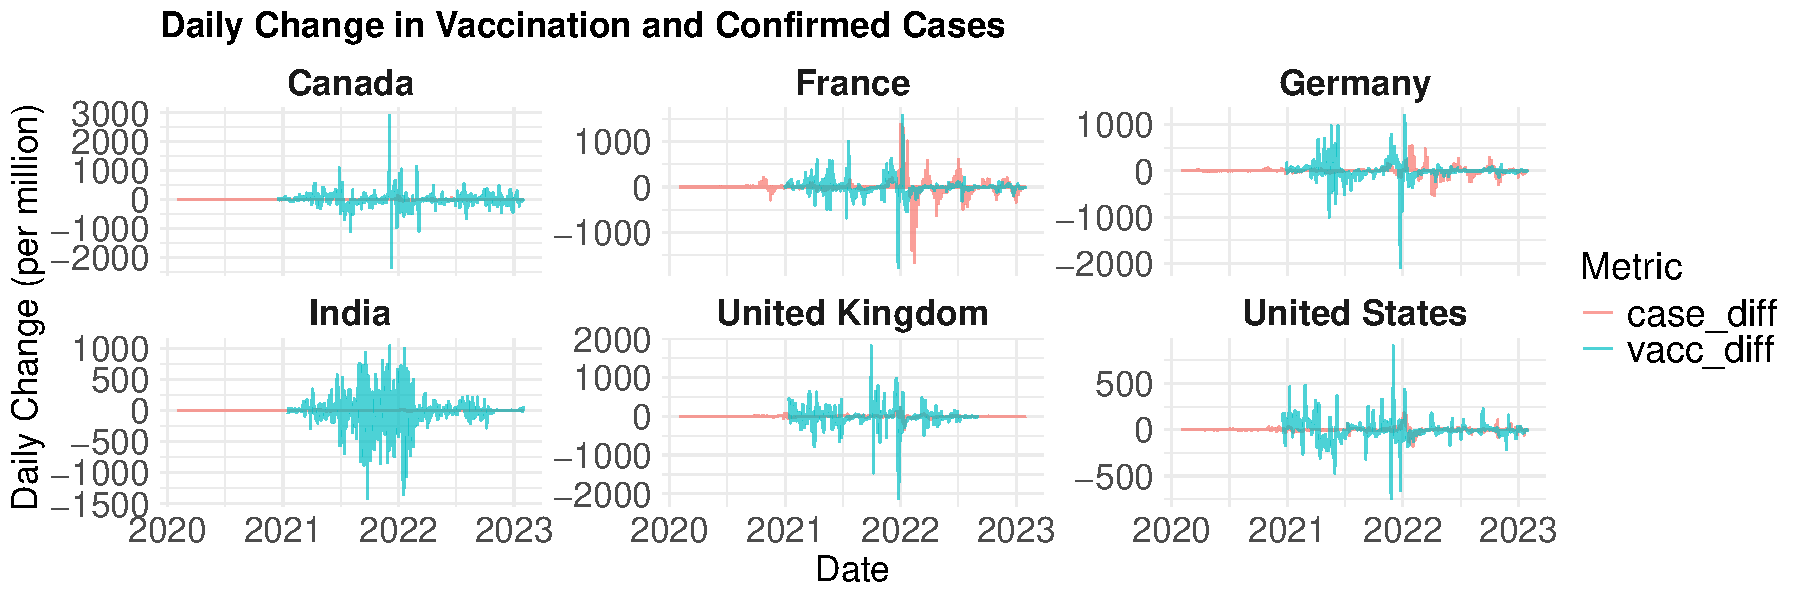
\includegraphics[keepaspectratio]{Analysis_files/figure-pdf/fig-daily-change-1.pdf}}

}

\caption{\label{fig-daily-change}Figure: Daily changes in confirmed
cases and vaccine doses per million}

\end{figure}%

Figure~\ref{fig-daily-change} highlights the daily change in confirmed
cases and vaccinations. It shows how much each number went up or down
each day. We can see during major outbreaks, the daily changes were
large. There were big increases in confirmed cases, and then some
countries also had big jumps in vaccination. This figure helps us
understand how fast things changed. It also shows how quickly some
countries reacted when cases increased.

\begin{figure}

\centering{

\pandocbounded{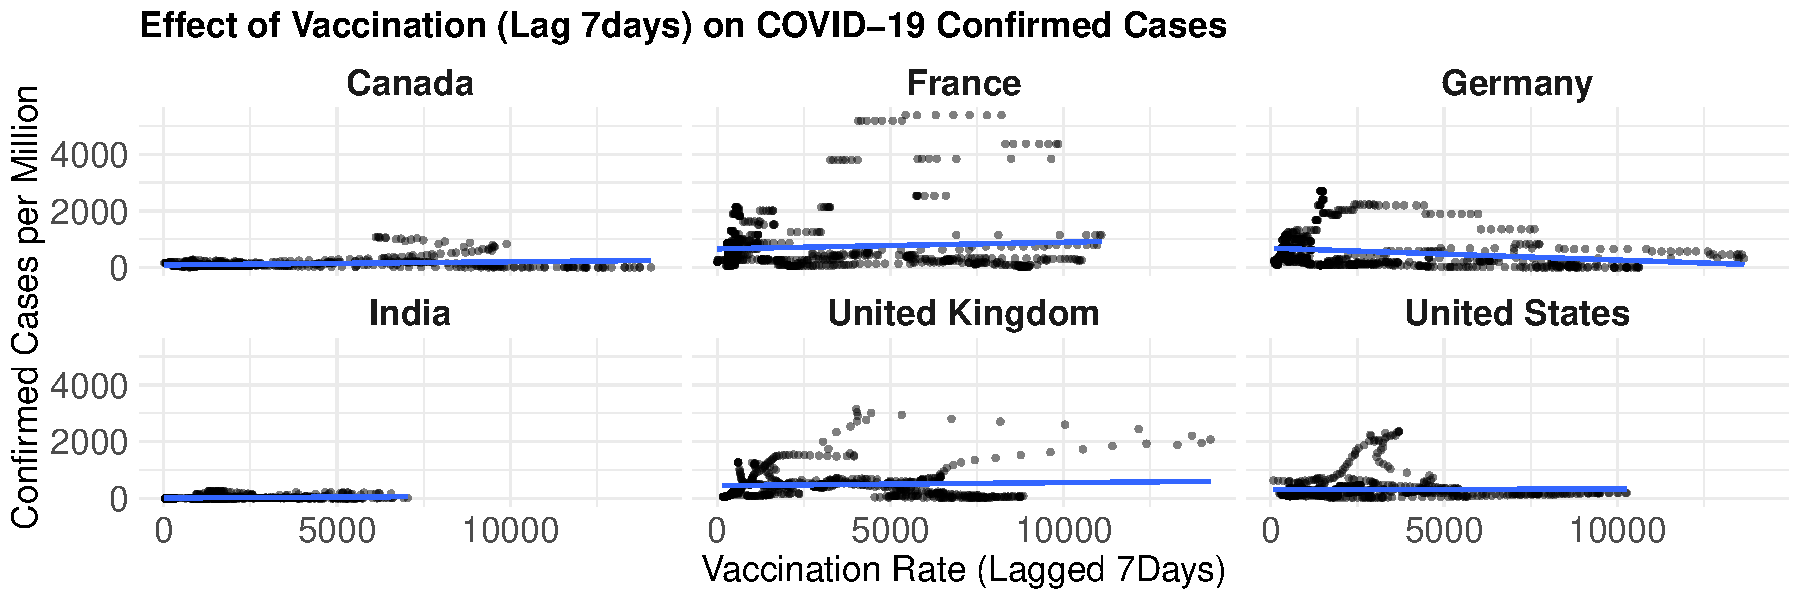
\includegraphics[keepaspectratio]{Analysis_files/figure-pdf/fig-lag-effect-1.pdf}}

}

\caption{\label{fig-lag-effect}Figure: Lagged vaccination rate vs
confirmed cases (7-day lag, by country)}

\end{figure}%

To understand if vaccines helped reduce new COVID-19 cases, we looked at
vaccination rates with a 7-day lag. This means we checked if higher
vaccination numbers one week earlier were linked to fewer new cases
later. The Figure~\ref{fig-lag-effect} shows that in countries like the
US and UK, when more people were vaccinated, new case numbers often went
down after a few days. This suggests that vaccines helped slow the
spread of the virus.

However, as Our World in Data points out, vaccines became less effective
in stopping infections over time, especially when new variants appeared.
Even so, they still helped reduce the number of serious cases and
deaths.

\begin{figure}

\centering{

\pandocbounded{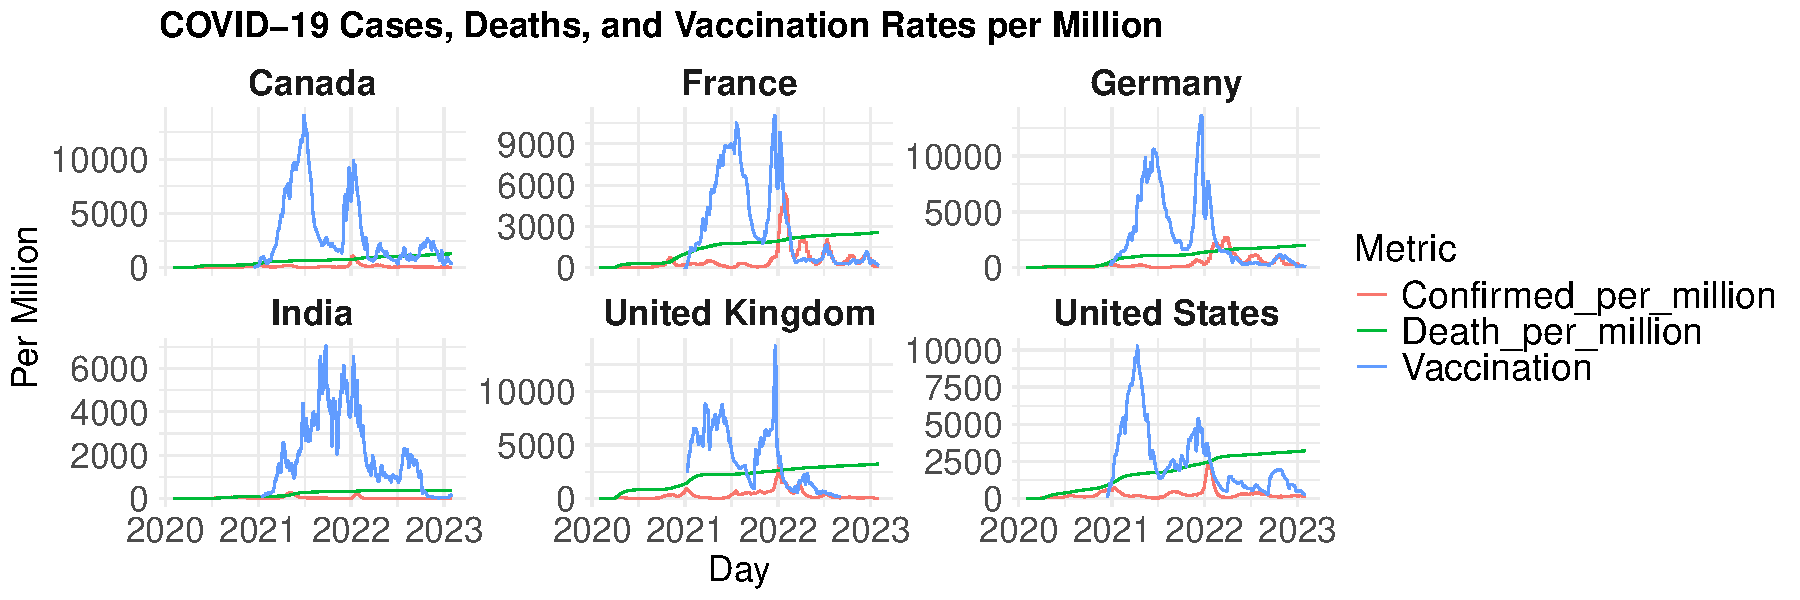
\includegraphics[keepaspectratio]{Analysis_files/figure-pdf/fig-case-death-vacc-1.pdf}}

}

\caption{\label{fig-case-death-vacc}Figure: COVID-19 confirmed
case-death rates-vaccination by country)}

\end{figure}%

Figure~\ref{fig-case-death-vacc} compares the trends of confirmed cases,
death rates, and vaccination rates across six countries. Earlier
waves---before widespread vaccination---showed a much closer link
between cases and deaths.

This pattern suggests that vaccination programs, alongside other public
health measures, played a key role in reducing the severity of outcomes
even when infection levels remained high.

The trend is less clear in countries with shorter or later vaccination
coverage, such as India, possibly due to data gaps or other healthcare
constraints.

We found that countries with early and wide vaccination had better
control of the virus. In these places, case numbers went down after
people started getting vaccinated. Later waves of COVID-19 caused fewer
deaths than early ones. This shows that vaccines helped not only to stop
the spread, but also to stop people from dying. Vaccination made a big
difference.

\section{Results}\label{sec-results}

The daily changes in COVID-19 case and vaccination rates in
Figure~\ref{fig-daily-change} shows that large outbreaks triggered
spikes in vaccination, indicating reactive public health responses.
Similarly, Figure~\ref{fig-vacc-vs-case}, shows that vaccines were often
given after case numbers had already started rising.

In early stages of the pandemic, before vaccination were widely
available, the number of deaths closely followed the number of confirmed
cases. However, as vaccination rates increased, the gap between cases
and deaths widened, suggesting that vaccines helped reduce the severity
of outcomes as per Figure~\ref{fig-case-death-vacc} illustrates trends
in confirmed COVID-19 cases, deaths, and vaccination rates per million
across six countries.

In countries like the United States and United Kingdom, higher
vaccination rates were often followed by declines in new case numbers.
This is also shown in Figure~\ref{fig-lag-effect}, which used a 7-day
delay to study the effect of vaccines. It suggests vaccines helped slow
down the spread of the virus soon after rollout.

The overall findings show that vaccination contributed to lower death
rates and reduced the impact of major outbreaks when implemented early
and consistently.

\section{Discussion}\label{sec-discussion}

\begin{enumerate}
\def\labelenumi{\arabic{enumi}.}
\tightlist
\item
  Case rates depend heavily on how much testing was available and how
  consistently it was used. Some countries, particularly in early stages
  of the pandemic, had limited testing capacity, meaning many infections
  may have gone unrecorded. In contrast, countries with widespread and
  frequent testing likely reported more cases, even among people with
  mild or no symptoms.
\item
  The differences in how countries report COVID-19 deaths may affect the
  accuracy of comparisons. For example, some countries may only record
  deaths that occur in hospitals, while others include deaths that
  happen at home. This means that countries with more limited reporting
  systems could appear to have lower death rates, even if the actual
  impact was higher.
\end{enumerate}

\section{Conclusion}\label{sec-conclusion}

During the project, we analyzed numbers of confirmed cases, deaths and
vaccinations in Canada, France, Germany, India, the UK and the US.

Our findings highlight three key observations:

\begin{enumerate}
\def\labelenumi{\arabic{enumi}.}
\item
  In most countries, the number of cases increased quite a bit before
  widespread vaccination took place.
\item
  During major outbreaks, both case numbers and vaccine doses
  administered showed significant daily fluctuations.
\item
  A 7-day lag analysis indicated that rising vaccination rates were
  followed by a reduction in new case numbers. Areas where vaccination
  started early and was kept up showed the strongest impact.
\end{enumerate}

These insights suggest that timely and sustained vaccination campaigns
played a crucial role in reducing transmission and saving lives. Future
public health responses should prioritize early vaccine deployment
during pandemics.

\section{Recommendations}\label{sec-recommendations}

Given the findings, we suggest that further pandemic responses
concentrate on spreading vaccinations quickly, especially in
lower-income parts of the world like India, in order to reduce chances
for breaks in case numbers. As seen in Figure~\ref{fig-daily-change},
rather than waiting for a surge, Governments should consider
establishing proactive vaccination schemes, ensuring vaccines are
deployed before a high number of cases occur. Having comparable ways of
reporting data in different nations allows for better assessment and
guides effective policy creation. Finally such campaigns need to make
sure vaccination efforts continue, because sustained work in the US and
UK greatly reduced the number of people affected and the death rate, as
shown in Figure~\ref{fig-case-death-vacc}.




\end{document}
